
\section{Vergleich des impliziten und expliziten Eulers}

In diesem Kaptiel gehts es darum die auswirkung der impliziten Löser auf die \textit{NeuralODE} zu analysieren.
Dazu wurden drei Bespiel-Trajektorien berechnet.
Welche jeweils mit dem impliziten und expliziten Euler berechnet wurde.
Um beide Verfahren möglichst gut miteinander Vergleichen zu können wurde, darauf geachtet das beide Verfahren mit den gleichen Einstellungen berechnet wurden.
Dies führt jedoch dazu, dass damit die expliziten Methoden
überhaupt ihre Trajektorie komplett berechenen können, 
die Fehler Werte auf einen Mindest-Wert gesetzt werden müssen.
Dies führt dazu, dass die impliziten Methoden ihre eigentlichen Stärken ihre Schrittweite so anzupassen 
dass diese das bestmögliche Ergebniss erreichen nicht 
voll ausnutzen können.
Werden nun die Fehler der beiden berechneten Trajektorien
direkt miteinander verglichen, kann kaum ein Unterschied erkannt werden.
Desshalb wird in der folgenden Grafik
die Differenz der impliziten und expliziten löser geplottet.

$$
d = e_{Implizit} - e_{Explizit}
$$

Dabei wurde explizit auf den Betrag verzichtet damit gesehen werden kann in welchem abschnitt welcher löser den geringeren fehler hat.
Ist also in der Folgenden Grafik die Differenz positiv 
ist der explizite Euler besser.
Im Negativen bereich hat dann der impliziten Euler den geringeren Fehler.

\begin{figure}
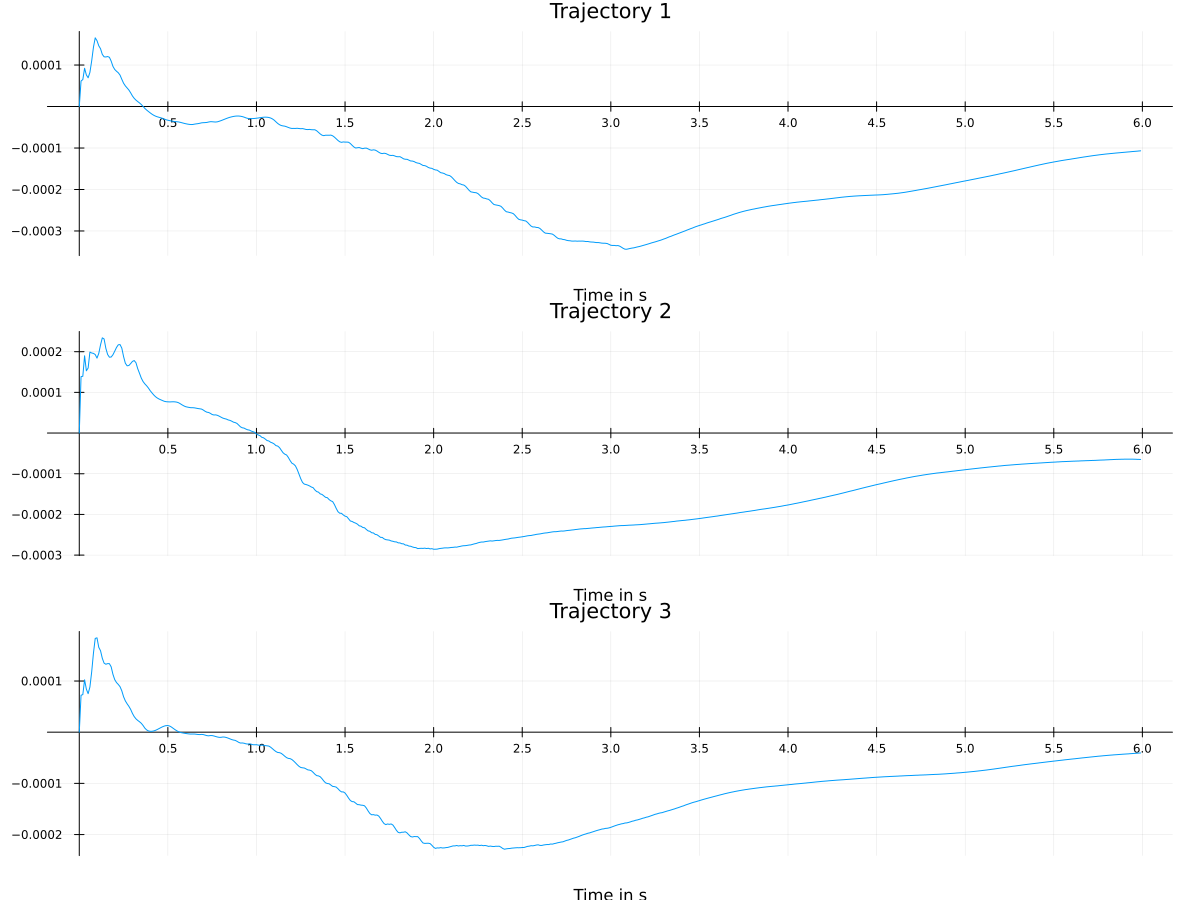
\includegraphics[width=\textwidth]{Data/03_Ergebnisse/errors.png}
\label{fig:eulervergleich}
\end{figure}

In der Graphic kann beobachtet werden, dass beim allen Trajektorien zuerst der explizite Euler das bessere Ergebniss liefert.
Dies liegt vor allem daran, dass es sich in unserem Beispiel 
um einen Flüssigkeits simulation handelt, welche mit einer laminaren Strömung begint.
Da diese sich sehr linear verhalten liefert der expliziten 
euler hier sehr gute Ergebnisse.
In der Simulation trifft das Wasser dann nach 0.5s bis 1s
auf ein Objekt.
Dies sorgt für mehr Turbulenzen im fluss der Flüssigkeit.
Ab diesem Zeitpunkt ist der implizite Euler besser.
Dies liegt vor allem daran, dass dieser mit nicht linearen Problemen besser zurecht kommt.
Es fällt ausserdem auf das sich beide Verfahren mit der Zeit
immer weiter annähern.
Dies liegt daran, dass im Allgemeinen mit der Zeit die Fehler der
Trajektorien immer größer werden.
Auch wenn es an hand der Daten nicht zeifels frei zu erkennen ist,
lassen die Daten vermuten, dass der implizite Euler auch bei längeren Trajektorien ein besseres Ergebniss liefert.
Obwohl die Daten klar zeigen, dass der Implizite Euler bessere
ergebnisse liefert, sollte dieser doch nicht immer gewählt werden.
Wie bereits angesprochen hängt die Qualität der Löser stark vom zu berechnedem Problem ab.
Der geringere Fehler der Trajektorie, benötigt jedoch eine deutlich
größere Laufzeit.
Bei den expliziten Methoden kann einen Laufzeit von ein paar Minuten 
erwartet werden. Beim impliziten Euler kommt es zu einer Laufzeit von einigen Tagen. 
In diesem Kapitel wurden die Vor- und Nachteil der beiden Methoden vorgestellt.
Wie diese zwei Verfahren miteinander verbunden werden können, geht es im nächsten Kapitel.
